\documentclass{article}

\usepackage{tikz}
\usetikzlibrary{graphs,quotes,arrows.meta}
\usetikzlibrary{automata,positioning}

\begin{document}

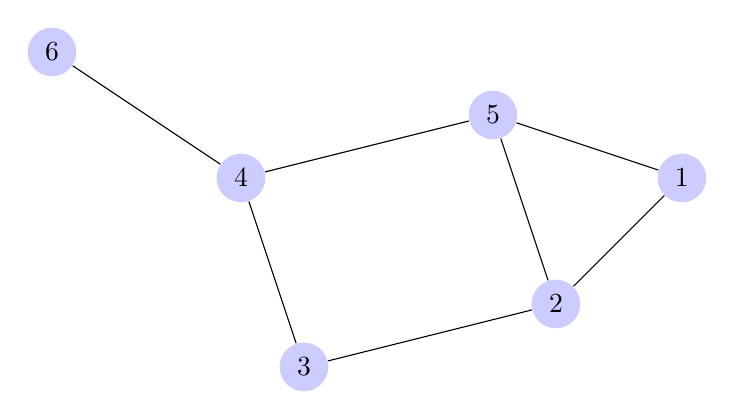
\begin{tikzpicture}
  [scale=.8,auto=left,every node/.style={circle,fill=blue!20}]
  \node (n6) at (1,10) {6};
  \node (n4) at (4,8)  {4};
  \node (n5) at (8,9)  {5};
  \node (n1) at (11,8) {1};
  \node (n2) at (9,6)  {2};
  \node (n3) at (5,5)  {3};

  \foreach \from/\to in {n6/n4,n4/n5,n5/n1,n1/n2,n2/n5,n2/n3,n3/n4}
    \draw (\from) -- (\to);

\end{tikzpicture}




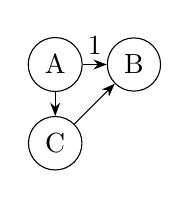
\begin{tikzpicture}
    \graph[nodes={draw,circle},edges={-{Stealth[]}}] {
      A -> ["1"] B, 
      A -> C,
      C -> B
    };
  \end{tikzpicture}




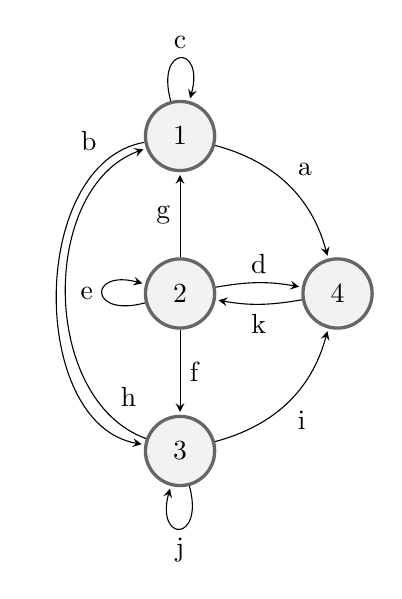
\begin{tikzpicture}%
  [>=stealth,
   shorten >=1pt,
   node distance=2cm,
   on grid,
   auto,
   every state/.style={draw=black!60, fill=black!5, very thick}
  ]
\node[state] (mid)                  {2};
\node[state] (upper) [above=of mid] {1};
\node[state] (right) [right=of mid] {4};
\node[state] (lower) [below=of mid] {3};

\path[->]
%   FROM       BEND/LOOP           POSITION OF LABEL   LABEL   TO
   (upper) edge[bend left]     node                      {a} (right)
           edge[bend right=80] node[swap,very near start]{b} (lower)
           edge[loop above]    node                      {c} (upper)
   (mid)   edge[bend left=10]  node                      {d} (right)
           edge[loop left]     node                      {e} (mid)
           edge                node                      {f} (lower)
           edge                node                      {g} (upper)
   (lower) edge[bend left=70]  node[swap,very near start]{h} (upper)
           edge[bend right]    node[swap]                {i} (right)
           edge[loop below]    node                      {j} (lower)
   (right) edge[bend left=10]  node                      {k} (mid)
   ;
\end{tikzpicture}








\end{document}